% siminos/CLE/symDyn.tex
% $Author$ $Date$

% symmetry in dynamical systems

We consider a system of \ode s of the form
\beq
	\dot{\ssp} = \vf(\ssp)
	\label{eq:difeq}
\eeq
where $\vf: \pS \rightarrow \pS$ a $C^\infty$ mapping and $\pS\subset\Rls{n}$
a manifold. Any compact Lie group acting on $\Rls{n}$ can be identified
with a subgroup of $\On{n}$, \cf\ for example \refref{golubII}
for a sketch of the proof. Therefore, without loss of generality
we will concentrate on subgroups $\Group\subseteq\On{n}$ in the following.
\ES{Can we generalize this to say that any compact Lie group acting on a
manifold can be can be identified with a subgroup of $\On{n}$ acting on $\Rls{n}$?}
Here the emphasis is on continuous symmetry, so we will restrict attention
to compact Lie groups. Moreover, we will restrict attention to the one parameter case.
Generalization to higher-dimensional groups is immediate.

We call a group element $\gamma\in\On{n}$ a symmetry of
\refeq{eq:difeq} if for every solution $x(t)$, $\gamma x(t)$
is also a solution. Equivalently $\gamma$ is a symmetry of \refeq{eq:difeq} if
\beq
	\vf(\gamma x) =\gamma \vf(x)
	\label{eq:equiv}
\eeq
for all $x\in\Rls{n}$. We say that $\vf$ \emph{commutes} with
$\gamma$ or that $\vf$ is $\gamma$-\emph{equivariant}. When
$\vf$ commutes with all $\gamma\in\Group$ we say that $\vf$
is $\Group$-equivariant. The finite time flow
$\flow{t}{\gamma x_o}$ through $\gamma x_o$ satisfies the
equivariance condition 
\beq\label{eq:equivFinite}
\flow{t}{\gamma x_o}=\gamma\flow{t}{x_o}
\eeq
from definition of symmetry and uniqueness of
solutions. In physics literature the term $invariant$ is most
commonly used, mostly because in Hamiltonian systems symmetry
is manifested as invariance of the Hamiltonian under the
symmetry operation\ES{To Predrag: Do you agree with this statement?}.

It can easily be checked that \CLe\ are equivariant under the one parameter rotation
group $\Un{1}\cong\SOn{2}$ acting by
\beq\label{eq:SO2cle}
	(x,\,y,\,z)\mapsto (e^{i\theta}x,\,e^{i\theta}y,\,z)\,,\ \theta\in[0,2\pi]\,.
\eeq
    \ES{In this representation equivariance is easy to check
    but here we should also discuss infinitesimal generator.}

In resemblance with a dynamical orbit, the \emph{group orbit} or $\Group$-orbit of 
$x\in\Rls{n}$ is the set
\beq
	\Group x = \{\Glmn x: \Glmn\in\Group\}\,
\eeq
of all points in which $x$ is mapped under the action of all group elements of $\Group$.

A set of group actions which maps a \statesp\ point $\ssp$ into itself,
\beq
\stab{\ssp} =\{\Glmn \in \Group: \Glmn \ssp = \ssp \}
    \,,
\ee{def:isotr}
is called the \emph{isotropy} (or \emph{stabilizer})  group of $\ssp$.
Thus the isotropy subgroup describes the symmetries of a point $x$. Note that by
definition the isotropy subgroup is the largest subgroup (in the
sense of set inclusion) that leaves $\ssp$ fixed.

We define the \emph{group of symmetries} of a set $X$ as the subgroup $\Subgroup_X$ that
leaves $X$ invariant as a set: 
\beq
	\Subgroup_X= {\Glmn: \Glmn X = X}\,. 
\eeq

The \emph{\fixedsp} of any subgroup $\Subgroup\subset\Group$,
denoted by $Fix(\Subgroup)$, is the subspace of $\Manif$ containing all fixed points of $\Sigma$:
\[
	Fix(\Sigma)=\{x\in\Manif\ |\ \sigma x = x\,,\ \forall \sigma\in\Sigma\}\,.
\]

\Fixedsp s are invariant under $\Group$-equivariant dynamics, $f^t\left(Fix(\Sigma)\right)\subseteq Fix(\Sigma)$
for all $t$. Therefore if $x(t)$ is a solution trajectory of an equivariant ODE then
$\stab{x(t)}=\stab{x(0)}$ for all $t$. See, for example,\rf{golubitsky2002sp} for proofs.

In the following it will be useful to introduce the
notion of a \emph{\csection}, an $(n-r)$-dimensional submanifold $K$
of $\Manif$ such that $K$ intersects each group orbit
transversally and at most once\ES{If ``at most once'' part holds Fels
and Olver\rf{FelsOlver99} call this a regular (local) cross-section,
otherwise a (local) cross-section}. In other words, 
\csection\ is a Poincar\'e section for group
orbits. As is the case for the dynamical Poincar\'e sections, in
general a single \csection\ does not suffice to intersect all group
orbits of points in \pS. This is rather surprising for linear groups and
to be able to understand this fact we will need to introduce some more
group theoretical notions that are related to the way groups act on $\pS$.
\ES{dropped:
We say that $\Group$ acts locally freely on \pS\ if for any $x\in\pS$ the
isotropy subgroup $\stab{x}$ is a discrete subgroups of $\Group$.
An r-dimensional compact Lie group $\Group$ acts \emph{locally freely} on $\pS$
if and only if it has $r-dimensional$ orbits\rf{FelsOlver99}.  
A group $\Group$ acts freely on $\pS$ if all isotropy subgroups 
are trivial: \stab{x}=\{e\} for all $x\in \Manif$.
If in addition for each point $x\in \Manif$ 
there exists an arbitrarily small neighborhood $U$ such that each 
orbit of $\Group$ intersects $U$ in a pathwise connected subset, 
then the group acts regularly.
}

A group $\Group$ acts semi-regularly on $\pS$ if all its orbits have 
the same dimension. Therefore the group orbits of a group that
acts semi-regularly foliate $\pS$. 
\ES{dropped: Note that locally free action implies
semi-regular action. 
}

The systems that we study here are not associated with a
variational principle. Therefore Noether's theorem does not
apply and we  cannot conclude the existence of a conserved
quantity associated with a continuous symmetry of the system.
Such a conserved quantity would restrict dynamical
trajectories to an invariant manifold locally transverse to
the direction of group action. In the contrary here the
system also evolves along the direction of group action. In
the example of {\CLe} this is demonstrated in
\reffig{fig:CLE}, where we project trajectories in
$(x_1,x_2,z)$ axes, where $x=x_1+ i\, x_2\,,\ y=y_1+i\, x_2$
with $x_i,\,y_i\in\Rls{}$. A generic trajectory slowly ``drifts'' 
along the direction of rotations while tracing a Lorenz-butterfly
like attractor. 
\ES{dropped as it is discussed elsewhere:
\refFig{fig:CLE} also
illustrates the need for continuous symmetry reduction as a
prerequisite for an understanding of state space geometry of
such systems. Symmetry related points can be considered equivalent
and identified. Until one proceeds with this identification, \ie\ before
symmetry reduction, any notion of distance is not useful in identifying recurrence.
}


\subsection{Solutions of systems with continuous symmetry}

A complete clasification of solutions in systems with continuous symmetries is
beyond the scope of this paper. Here we concentrate on particular types of solutions
that play an important dynamical role in the examples we will consider and also
help explain the need for symmetry reduction.

In contrast to \emph{\eqv} solutions that satisfy
$f^\tau(\ssp) - \ssp = 0$, \emph{\reqva} satisfy $f^\tau(\ssp) -
\LieEl( \tau) \, \ssp= 0$ for any $\tau$. In a co-moving frame, \ie, a frame moving 
along the group orbit with velocity
$\vel(\ssp) = \velRel \cdot \groupTan(\ssp)$\ES{define $\groupTan$ in symmetry section, choose
a pretier symbol}, the \reqv\ appears as an \eqv.

A {\em \rpo} $p$ is an orbit $\pS_p$ in {\statesp} $\pS$
which exactly recurs
    \index{periodic!orbit!relative}\index{relative!periodic orbit}
\beq
\ssp_p (0) = \LieEl_p \ssp_p (\period{p} )
    \,,\qquad
\ssp_p (\tau) \in \pS_p
    \,,
\label{RPOrelper1}
\eeq
at a fixed {\em relative period} $\period{p}$, but
shifted by a fixed group action ${\LieEl_p}$
which brings the endpoint $\ssp_p (\period{p} ) $
back into the initial point $\ssp_p (0) $, see \reffig{f:rpo}.
The group action ${\LieEl_p}$ parameters
$\gSpace = (\gSpace_1,\gSpace_2,\cdots\gSpace_N)$
will be referred to as ``phases,'' or ``shifts.''
% In contrast to the pre-periodic \refeq{preperiodic}, 
The phases here are irrational, and the trajectory sweeps out
ergodically the group orbit without ever closing into a \po.
For dynamical systems with only continuous (no discrete)
symmetries, the parameters $\{t,\gSpace_1,\cdots,\gSpace_N\}$
are real numbers, ratios $\pi/\gSpace_j$ are almost never
rational, the likelihood of finding a {\po} for such system is
{zero}, and such \rpo s are almost never eventually periodic.

%
%%%%%%%%%%%%%%%%%%%%%%%%%%%%%%%%%%%%%%%%%%%%%%%%%%%%%%%%%%%%%%%%
% hand-drawn in dasbuch/book/FigSrc/xfig/rpo.fig
\begin{figure}[ht]
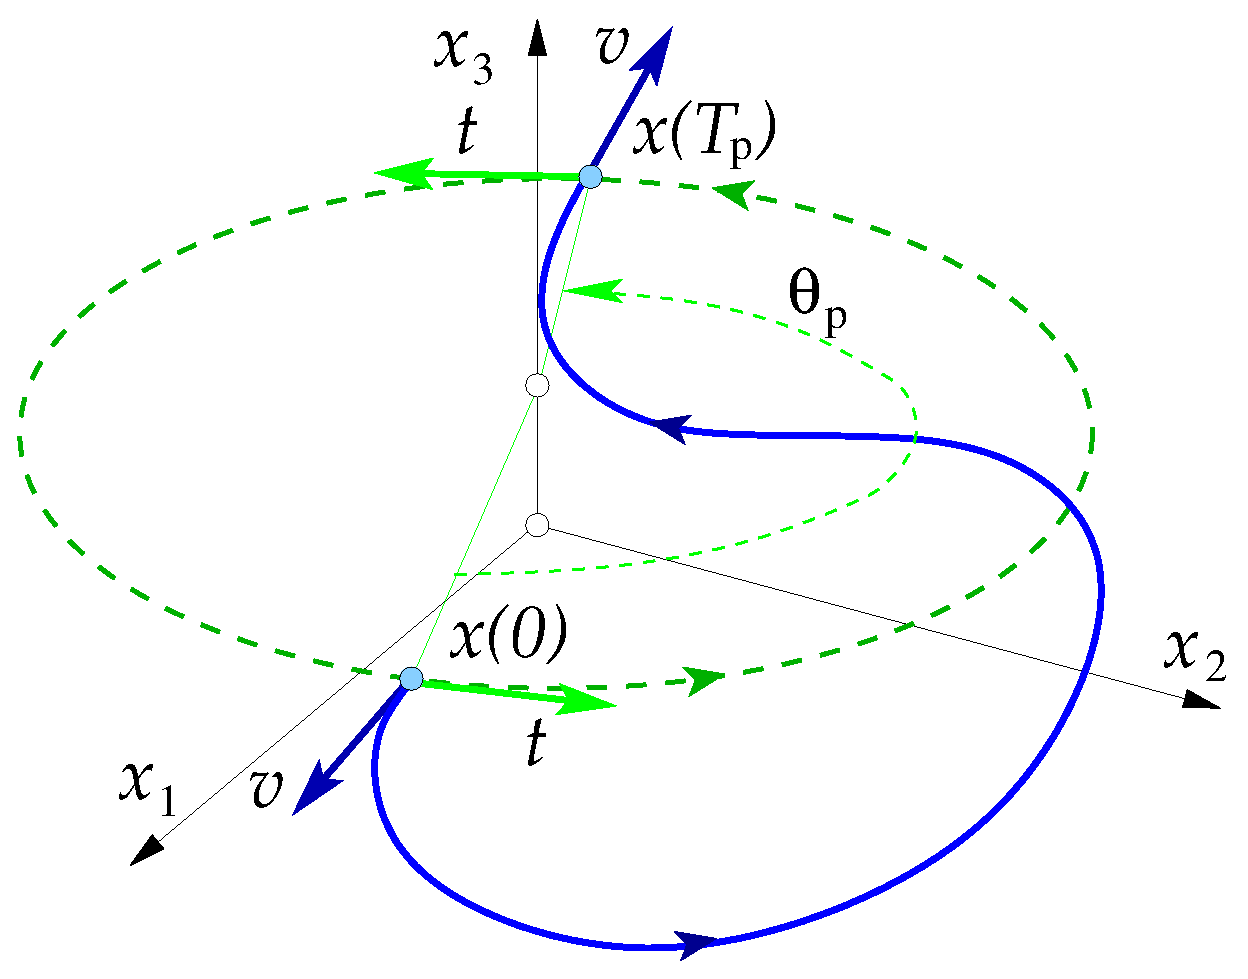
\includegraphics[width=0.5\textwidth]{../figs/rpo.eps}
\caption{
A \rpo\ starts out at $\ssp(0)$ with the dynamical $\vel$ and
group tangent $\groupTan$ flows pointing in different
directions, and returns to the group orbit of $\ssp(0)$ after
time $\period{p}$ at $\ssp(\period{p})=\LieEl_p \ssp (0)$, a
rotation of the initial point by $\LieEl_p$.
}
\label{f:rpo}
\end{figure}
%%%%%%%%%%%%%%%%%%%%%%%%%%%%%%%%%%%%%%%%%%%%%%%%%%%%%%%%%%%%%%%%%%

Similarly to a \reqv, a \emph{\rpo} is periodic in its
mean velocity $\velRel_p=\gSpace_p/\period{p}$ co-rotating
frame (see \reffig{f:MeanVelocityFrame}), but in the
stationary frame its trajectory is quasiperiodic. 
A co-moving
frame is helpful in visualizing a single `relative' orbit,
but useless for viewing collections of orbits, as each one
drifts with its own angular velocity. Visualization of all
\rpo s as \po s we attain only by global symmetry reduction,
to be undertaken in \refsect{s:symRedGeneral}.


\ES{move elsewere: The lowest level of organization of the
familiar (real) Lorenz system that does not posses a
continuous symmetry can be
understood\rf{DasBuch,SiminosThesis} in terms of the unstable
manifolds of the equilibrium at the origin and the two
(discrete-symmetry-related) equilibria $\EQV{1,2}$. In the
case of {\CLe}  the origin \EQV{0} is an \eqv\ of
\refeq{eq:CLe} for any value of the parameters. As shown in
\refref{FowlerCLE82} it is stable for $0<\RerCLor<\rho_{1c}$
and unstable for $\rho_{1c}<\RerCLor$, where
\beq
	\rho_{1c} = 1 + \frac{(e+\ImrCLor)(e-\sigma \ImrCLor)}{(\sigma+1)^2}\,.
\eeq
At bifurcation a pair of eigenvalues crosses the imaginary axis with imaginary part:
\beq
	\omega_c = \frac{\sigma (e + \ImrCLor)}{\sigma+1}\,.
	\label{eq:omegaCLE}
\eeq
and a \emph{relative equilibrium} \REQV{}{1}, an equilibrium
in a frame rotating with constant angular velocity is born.
Alternatively we might say that a relative equilibrium is a
periodic orbit that is invariant (as a set) under the action
of $\LGelement{l_p}\in\Group$ for any $l_p$.
    \ES{this implies constant angular velocity by
    equivariance.}
    \ES{Does not fit here, but keep: For $e+\ImrCLor=0$ the
    relative equilibrium degenerates to an \SOn{2}-orbit of
    \eqva\rf{FowlerCLE82}, since $\omega_c =0$.}
As we will see in \refsect{s:StabReq}, \REQV{}{1} of {\CLe}
for the parameter set we study here is unstable with one
complex expanding eigenvalue. Yet, being a periodic orbit,
its unstable manifold is three-dimensional, with one
eigendirection corresponding to the direction of $\vf$ which
also coinsides with the direction of rotations of the system.
In \reffig{fig:CLE} we plot one trajectory on the unstable
manifold of \REQV{}{1}. While it spirals away from
$\REQV{}{1}$ it also ``drifts'' along the direction of
rotations of the system. This drifting motion obscures
understanding of the stretching mechanism along the expanding
eigendirection and subsequently the folding of the unstable
manifold back to itself.
}
%
%%%%%%%%%%%%%%%%%%%%%%%%%%%%%%%%%%%%%%%%%%%%%%%%%%%%%%%%%%%%
\begin{figure}[ht]
\begin{center}
  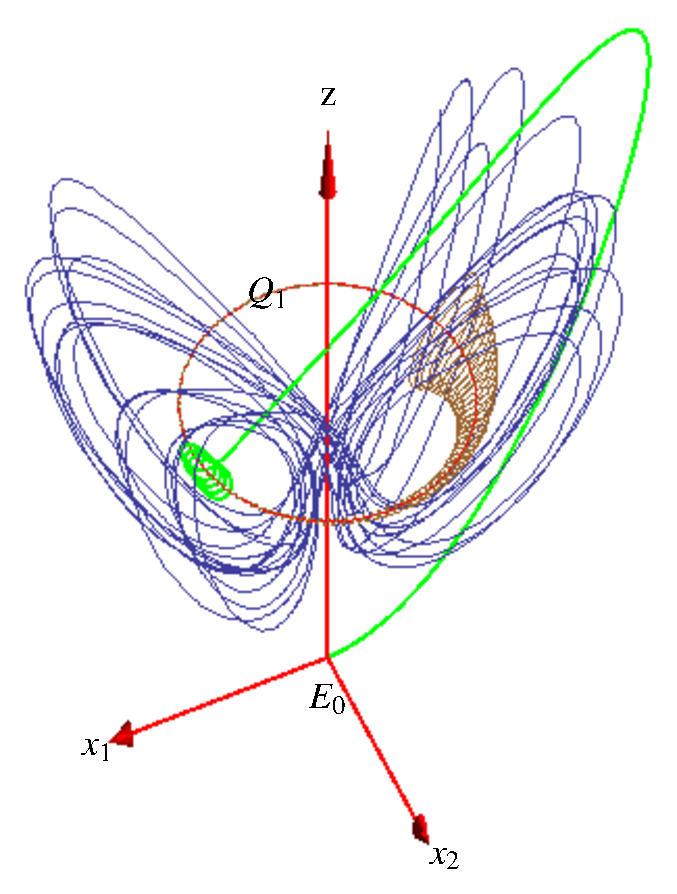
\includegraphics[height=0.25\textheight]{../figs/CLE}
\end{center}
\caption[Complex Lorenz flow phase space]
{ \Statesp\ portrait of \CLe\ dynamics for $e=1/10,\,
\ImrCLor=0$. Plotted are \reqv\ \REQV{}{1} (red), its unstable
manifold (brown), \eqv\ \EQV{0}, a representative of its
unstable manifold (green), 3 repetitions of \rpo\
``01''(magenta) and a generic orbit (blue).}
\label{fig:CLE}
\end{figure}
%%%%%%%%%%%%%%%%%%%%%%%%%%%%%%%%%%%%%%%%%%%%%%%%%%%%%%%%%%%%
%


\ES{move elsewere: The next (or a complimentary) level of organization of (real)
{\Le} attractor is provided by the dense set of \po s
embedded in it\rf{DV03,DasBuch}. In {\CLe} a secondary
bifurcation from \REQV{}{1} is expected, according to Krupa's
theorem\rf{Krupa90}, to result in \emph{relative periodic
orbits} that satisfy
\beq
	\LGelement{l_p}x(t+T_p)=x(t)\,,
\eeq
{\ie} they ``return'' after a time period $T_p$ to a point
that maps to the initial one under a group transformation
$\LGelement{l_p}$ with group parameter period $l_p$. A {\rpo}
of {\CLe} is shown in \reffig{fig:CLE} as its iterations fill
a torus. Therefore we see that in systems with continuous
symmetry we have to account for tori instead of {\po s} as
the organizational blocks of the attractor.
}

\PublicPrivate{}{
 \refFig{fig:CLE} illustrates the need
 to project dynamics on \reducedsp: Dynamics is organized by
 the interplay of the stable and unstable manifolds of \eqv\
 \EQV{0} and \reqv\ \REQV{}{1} but the dynamics along the
 direction of rotation blur the picture and the notion of
 recurrence becomes relative. We will present various
 approaches to orbit space reduction in the following.
% sections.
    }


\subsection{\CLe\ \reqva}

To find the location of the \reqv\ it is convenient to work
on polar coordinates defined by $x=r_1 e^{i \phi_1},\,y=r_2
e^{i \phi_2}$. Equations \refeq{eq:CLe} take the form
    %PC: Rebecca and I rederived these: they check.
\beq
\begin{split}
	\dot{r}_1 &=-\sigma (r_1 - r_2\cos\phi) \cont
	\dot{r}_2 &=-r_2 + r_1(\RerCLor -z)(\cos\phi-\ImrCLor\sin\phi) \cont
	\dot{z} &=  -b z+r_1 r_2\cos\phi \cont	
	\dot{\phi} &=-e-\frac{\sigma r_2 \sin\phi}{r_1}-\frac{r_1(\RerCLor-z) (\ImrCLor\cos\phi+\sin\phi) }{r_2}\,,
	\label{eq:CLePolar}
\end{split}
\eeq
where $\phi=\phi_1-\phi_2$ and the evolution equations for
$\phi_1,\phi_2$ are given by
\beq
\begin{split}
	\dot{\phi}_1 &=-\frac{\sigma r_2 \sin\phi}{r_1}\cont
	\dot{\phi_2} &= e +\frac{r_1\left( (\RerCLor -z)\sin\phi+\ImrCLor\cos\phi\right)}{r_2}\,.
	\label{eq:CLeAngl}
\end{split}
\eeq

For simplicity we now turn to the ``laser case''
$e\neq0,\;\ImrCLor=0$; in the numerical examples we set the
detuning to $e=1/10$.

The condition for a \reqv~ is that all time derivatives in
\refeq{eq:CLePolar} vanish from which we get
% Explicit form here, simplified in terms of z component below
% \beq
% \begin{split}
% 	z &= -\frac{e^2}{(\sigma +1)^2}+\RerCLor -1\cont
% 	r_2 &= \frac{\sqrt{-b \left(e^2+(\sigma +1)^2\right)\left(e^2-(\RerCLor -1) (\sigma +1)^2\right)}}{(\sigma+1)^2}\cont
% 	r_1 &= \frac{\sqrt{-b \left(e^2-(\RerCLor -1) (\sigma +1)^2\right)}}{\sigma +1}\cont
% 	\Phi &= -\cos ^{-1}\left(\frac{\sigma +1}{\sqrt{e^2+(\sigma +1)^2}}\right)
% \end{split}
% \eeq
\beq
\begin{split}
	z^{(1)} &= \frac{-e^2+(\RerCLor -1)(\sigma +1)^2}{(\sigma +1)^2}\cont
	r_1^{(1)} &= \sqrt{b z^{(1)}}\cont
	r_2^{(1)} &= \sqrt{b \left(e^2+(\sigma +1)^2\right)z^{(1)}}\cont
	\phi^{(1)} &= -\cos ^{-1}\left(\frac{\sigma +1}{\sqrt{e^2+(\sigma +1)^2}}\right)
\end{split}
\eeq
Substituting in \refeq{eq:CLeAngl} we get $\dot{\phi}_1=\dot{\phi}_2=e \sigma/(1 + \sigma)\neq 0$ for $e\neq0$
and thus we have indeed a \reqv, not a group orbit of \eqva.

Calculation  in polar coordinates $r_1,r_2,\phi,z$ of stability eigenvalues for \REQV{}{1}
for the set of parameters we use here yields
\beq
	\eigRe[1]\pm i\eigIm[1]= 0.0938\pm 10.1945i,\,
    \eigExp[3]=-11.0009,\, \eigExp[4]= -13.8534\,.
	\label{eq:CLeREQBstab}
\eeq


